%%% Einfaches Template für einen Abschlussbericht zum Berufspraktikum
%%% äöüÄÖÜß  <-- keine deutschen Umlaute hier? UTF-faehigen Editor verwenden!

%%% Magic Comments zum Setzen der korrekten Parameter in kompatiblen IDEs
% !TeX encoding = utf8
% !TeX program = pdflatex 
% !TeX spellcheck = de_DE
% !BIB program = biber

\RequirePackage[utf8]{inputenc} % bei Verw. von lualatex oder xelatex entfernen!
\RequirePackage{hgbpdfa}        % Erzeugt ein PDF/A-2b-konformes Dokument

\documentclass[internship,german,smartquotes,alphabetic]{hgbthesis}
% Zulässige Optionen in [..]: 
%    Typ der Arbeit: 'diploma', 'master' (default), 'bachelor', 'internship'
%		 Zusätzlich für ein Thesis-Exposé: 'proposal' (für 'bachelor' und 'master')
%    Hauptsprache: 'german' (default), 'english'
%    Option zur Umwandlung in typografische Anführungszeichen: 'smartquotes'
%    APA Zitierstil: 'apa'
%%%-----------------------------------------------------------------------------

\graphicspath{{images/}}  % Verzeichnis mit Bildern und Grafiken
\logofile{logo}           % Logo-Datei: images/logo.pdf (kein Logo: \logofile{})
\bibliography{references} % Biblatex-Literaturdatei (references.bib)

\usepackage{hyperref}
\usepackage[acronym]{glossaries}

\makeglossaries

\newacronym{jvm}{JVM}{Java Virtual Machine}
\newacronym{vt}{VT}{Virtual Thread}
\newacronym{pt}{PT}{Plattform Thread}
\newacronym{ot}{OT}{Betriebssystem Thread}
\newacronym{sts}{STS}{StructuredTaskScope}                          % makeglossaries main in der cmd ausführen
% \makeglossaries                           % makeglossaries muss dadurch nicht mehr in der cmd ausgeführt werden  


%%%-----------------------------------------------------------------------------
\begin{document}
%%%-----------------------------------------------------------------------------

%%%-----------------------------------------------------------------------------
% Angaben für die Titelei (Titelseite, Erklärung etc.)
%%%-----------------------------------------------------------------------------

% \title{Endbericht zum Berufspraktikum bei Mogulovich International}
% \author{Alex A.\ Schlaumeier}

% \programtype{Fachhochschul-Bachelorstudiengang}

% \programname{Medientechnik und -design}
% \placeofstudy{Hagenberg}

% \dateofsubmission{2024}{06}{25}
% \advisor{Pjotr I.~Czar, M.A.}
% \companyName{%
%    Mogulovich International Media GmbH\\
%    Online Division\\
%    Hubertusgasse 3a, 1020 Wien
% }
% \companyUrl{www.mogul.at}
\pagenumbering{alph}                    % damit die Titelseite mit 'a' beginnt und links wieder richtig funktionieren
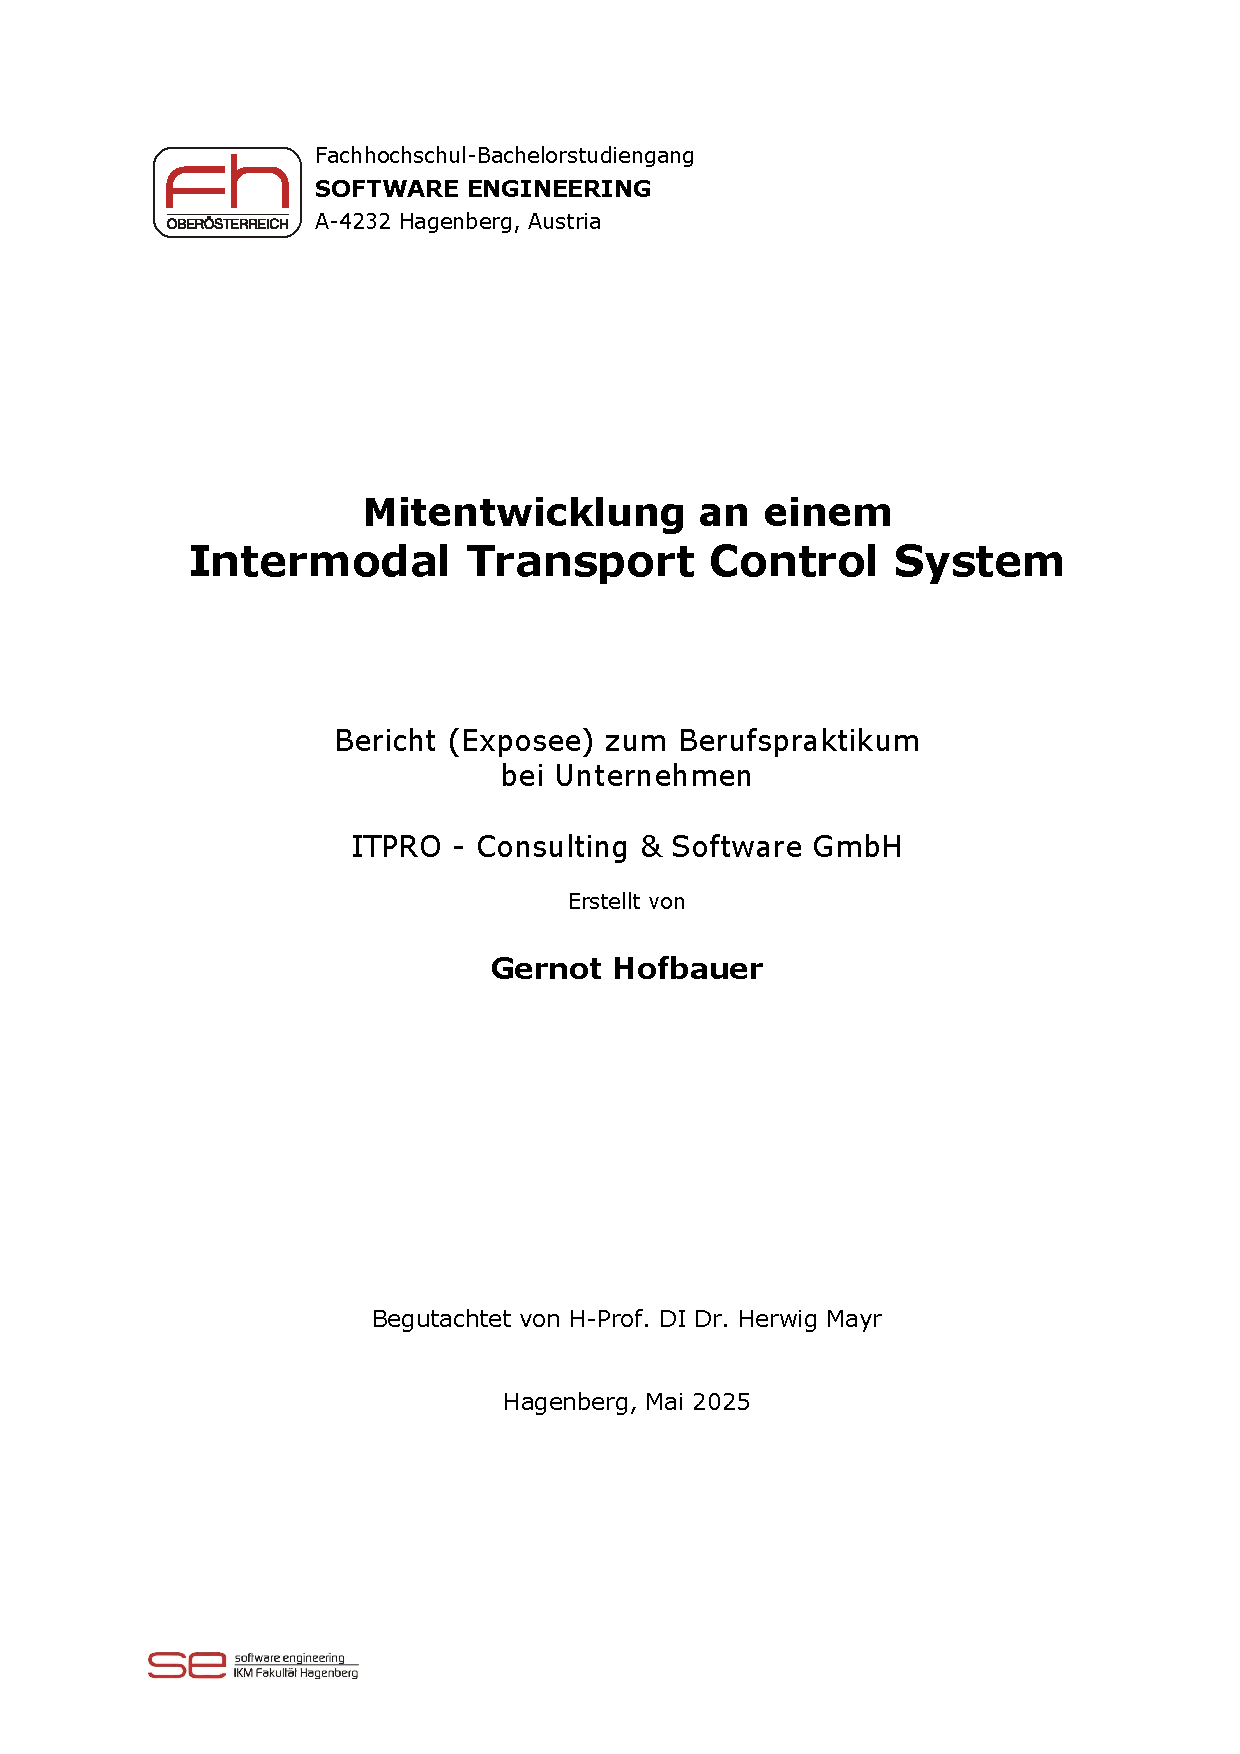
\includepdf[pages=-]{Titelblatt.pdf}
%%%-----------------------------------------------------------------------------
\frontmatter                                       % Titelei (röm. Seitenzahlen)
%%%-----------------------------------------------------------------------------

% \maketitle
\tableofcontents
\printglossary[type=\acronymtype,title=Akronyme]

%%%-----------------------------------------------------------------------------

\chapter{Kurzfassung}% Umfang der Kurzfassung: ca.\ 200 Worte.
Dieser Praktikumsbericht beschreibt die Arbeit des Praktikanten im Rahmen seines Praktikums bei der Firma ITCS GmbH. Der Schwerpunkt lag auf der Entwicklung
von Software für das ITCS-Management-System, das in der öffentlichen Verkehrsinfrastruktur eingesetzt wird. Das Herzstück dieser Software ist eine Webanwendung,
die es ermöglicht, Umläufe aus einzelnen Fahrten zu erstellen. Dabei sollten verschiedene benötigte Daten auf der darunterliegenden Datenbank generiert werden.
Außerdem sollten diese Umläufe auch automatisch auf Durchführbarkeit geprüft werden.
In diesem Praktikum wurde mit der Programmiersprache \emph{C\#} und dem \emph{.NET}-Framework gearbeitet. Der Datenbankzugriff erfolgte über die \emph{Entity Framework Core}-Bibliothek, 
die eine objektorientierte Abstraktionsebene für den Datenbankzugriff bereitstellt. Das Frontend wurde mit \emph{Blazor} entwickelt, einer modernen Webtechnologie, 
die es ermöglicht, interaktive Webanwendungen mit C\# zu erstellen. Durch die Verwendung von \emph{Blazor} konnte eine nahtlose Integration zwischen Frontend und Backend erreicht werden,
was die Entwicklung effizienter und flexibler machte.
Während der Implementierung diese Umlaufeditors musste auch teilweise das bestehende Datenmodell angepasst werden, um die neuen Anforderungen zu erfüllen. 
Da die Datenbank mit Daten aus anderen Systemen gefüllt wird, musste auch ein anderes, bestehendes Projekt, das für den Import und Export von Daten benutzt ist, angepasst werden.
Dabei musste darauf geachtet werden, dass die Daten weiterhin mit dem \emph{VDV-452}-Standard kompatibel bleiben, um die Interoperabilität mit anderen Systemen zu gewährleisten.

%%%-----------------------------------------------------------------------------
\mainmatter                             % Hauptteil (ab hier arab. Seitenzahlen)
%%%-----------------------------------------------------------------------------
\chapter{Einleitung}
\label{cha:Einleitung}

    Seit einigen Jahren Arbeitet Oracle an Möglichkeiten zur Verbesserung der Skalierbarkeit von Java-Anwendungen im Projekt "Loom".
    Der Hauptansatz dieses Vorhabens ist die Einführung von virtuellen Threads, die von der JVM verwaltet werden. 
    Diese Threads sind leichtgewichtiger als klassische Plattform Threads und können in größerer Anzahl erzeugt werden.
    So können bestimmte Anwendungen mit hoher Nebenläufigkeit zukünftig effizienter gestaltet werden. Diese Bachelorarbeit 
    beleuchtet diese Technologien und stellt die Neuerungen dem bereits Bekanntem gegenüber.

\section{Ziel der Arbeit}
\label{sec:Ziel}

    Das Ziel dieser Bachelorarbeit ist es, die grundlegenden Eigenschaften und Limitierungen des bestehenden Thread-Konzepts zu untersuchen und die Motivationen für die Neuerungen
    durch Projekt Loom zu verstehen. Ein Überblick über Projekt Loom und die damit verbundenen Technologien wird gegeben, wobei der Schwerpunkt auf Virtual Threads liegt. 
    Die Arbeit soll zeigen, wie und in welchen Fällen diese Neuerungen in der Praxis angewendet werden können und welche neuen Möglichkeiten sich dadurch ergeben. 
    Es wird auch verdeutlicht, welche bestehenden Probleme der parallelen Ausführung durch die neuen Technologien nicht gelöst werden können. 
    Durch Benchmarks sollen Laufzeit und Speicherverbrauch unter verschiedenen Umständen analysiert werden, um daraus Schlüsse zu ziehen, 
    in welchen Fällen die neuen Technologien verwendet werden sollten und in welchen nicht. Als konkretes Ergebnis wird eine Sammlung kleinerer Programme erstellt, 
    die die neuen Technologien in Projekt Loom demonstrieren und die Unterschiede zu den bisherigen Technologien aufzeigen.




\chapter{Design}\label{chap:design}

    Da wie bereits erwähnt, die Projekte \emph{"ITCS-Management"} und \emph{"ITCS"} bereits existierten, waren das grundlegende Design und die technische Architektur bereits vorgegeben.
    Dies umfasst sowohl Aspekte wie die Transaktionsverwaltung der Datenbank, als auch Elemente im Frontend, wie die Navigation zwischen den Seiten oder die Farbpalette.

\section{"ITCS-Management"}\label{sec:itcs-management-design}
    Im Projekt \emph{"ITCS-Management"} wurde eine Vielzahl an kleineren Aufgaben erledigt. Dabei handelte es sich um Blazor-Seiten, die meist nur Datenbank-Entitäten tabellarisch
    darstellen und beschränktes Editieren ermöglichen sollten. Im Bericht selbst wird auf diese Aufgaben, aufgrund ihrer repetitiven Natur, nicht weiter eingegangen. Fokussiert wird  
    auf die größte Aufgabe in diesem Projekt namens \emph{"Umlaufeditor"}. 
    Ein Umlauf stellt dabei eine Sequenz von Fahrten dar, die von einem einzelnen Fahrzeug in einem Durchgang durchgeführt wird. Die Fahrten werden von den meisten Kunden in anderen 
    Systemen erstellt und sind mit dem Import neuer Versionen in der Datenbank schon vorhanden. Die Umläufe hingegen werden nicht in anderen Systemen definiert und sollen deswegen
    mit diesem Editor erstellt und angepasst werden. 
    \begin{figure}[H]
        \centering
        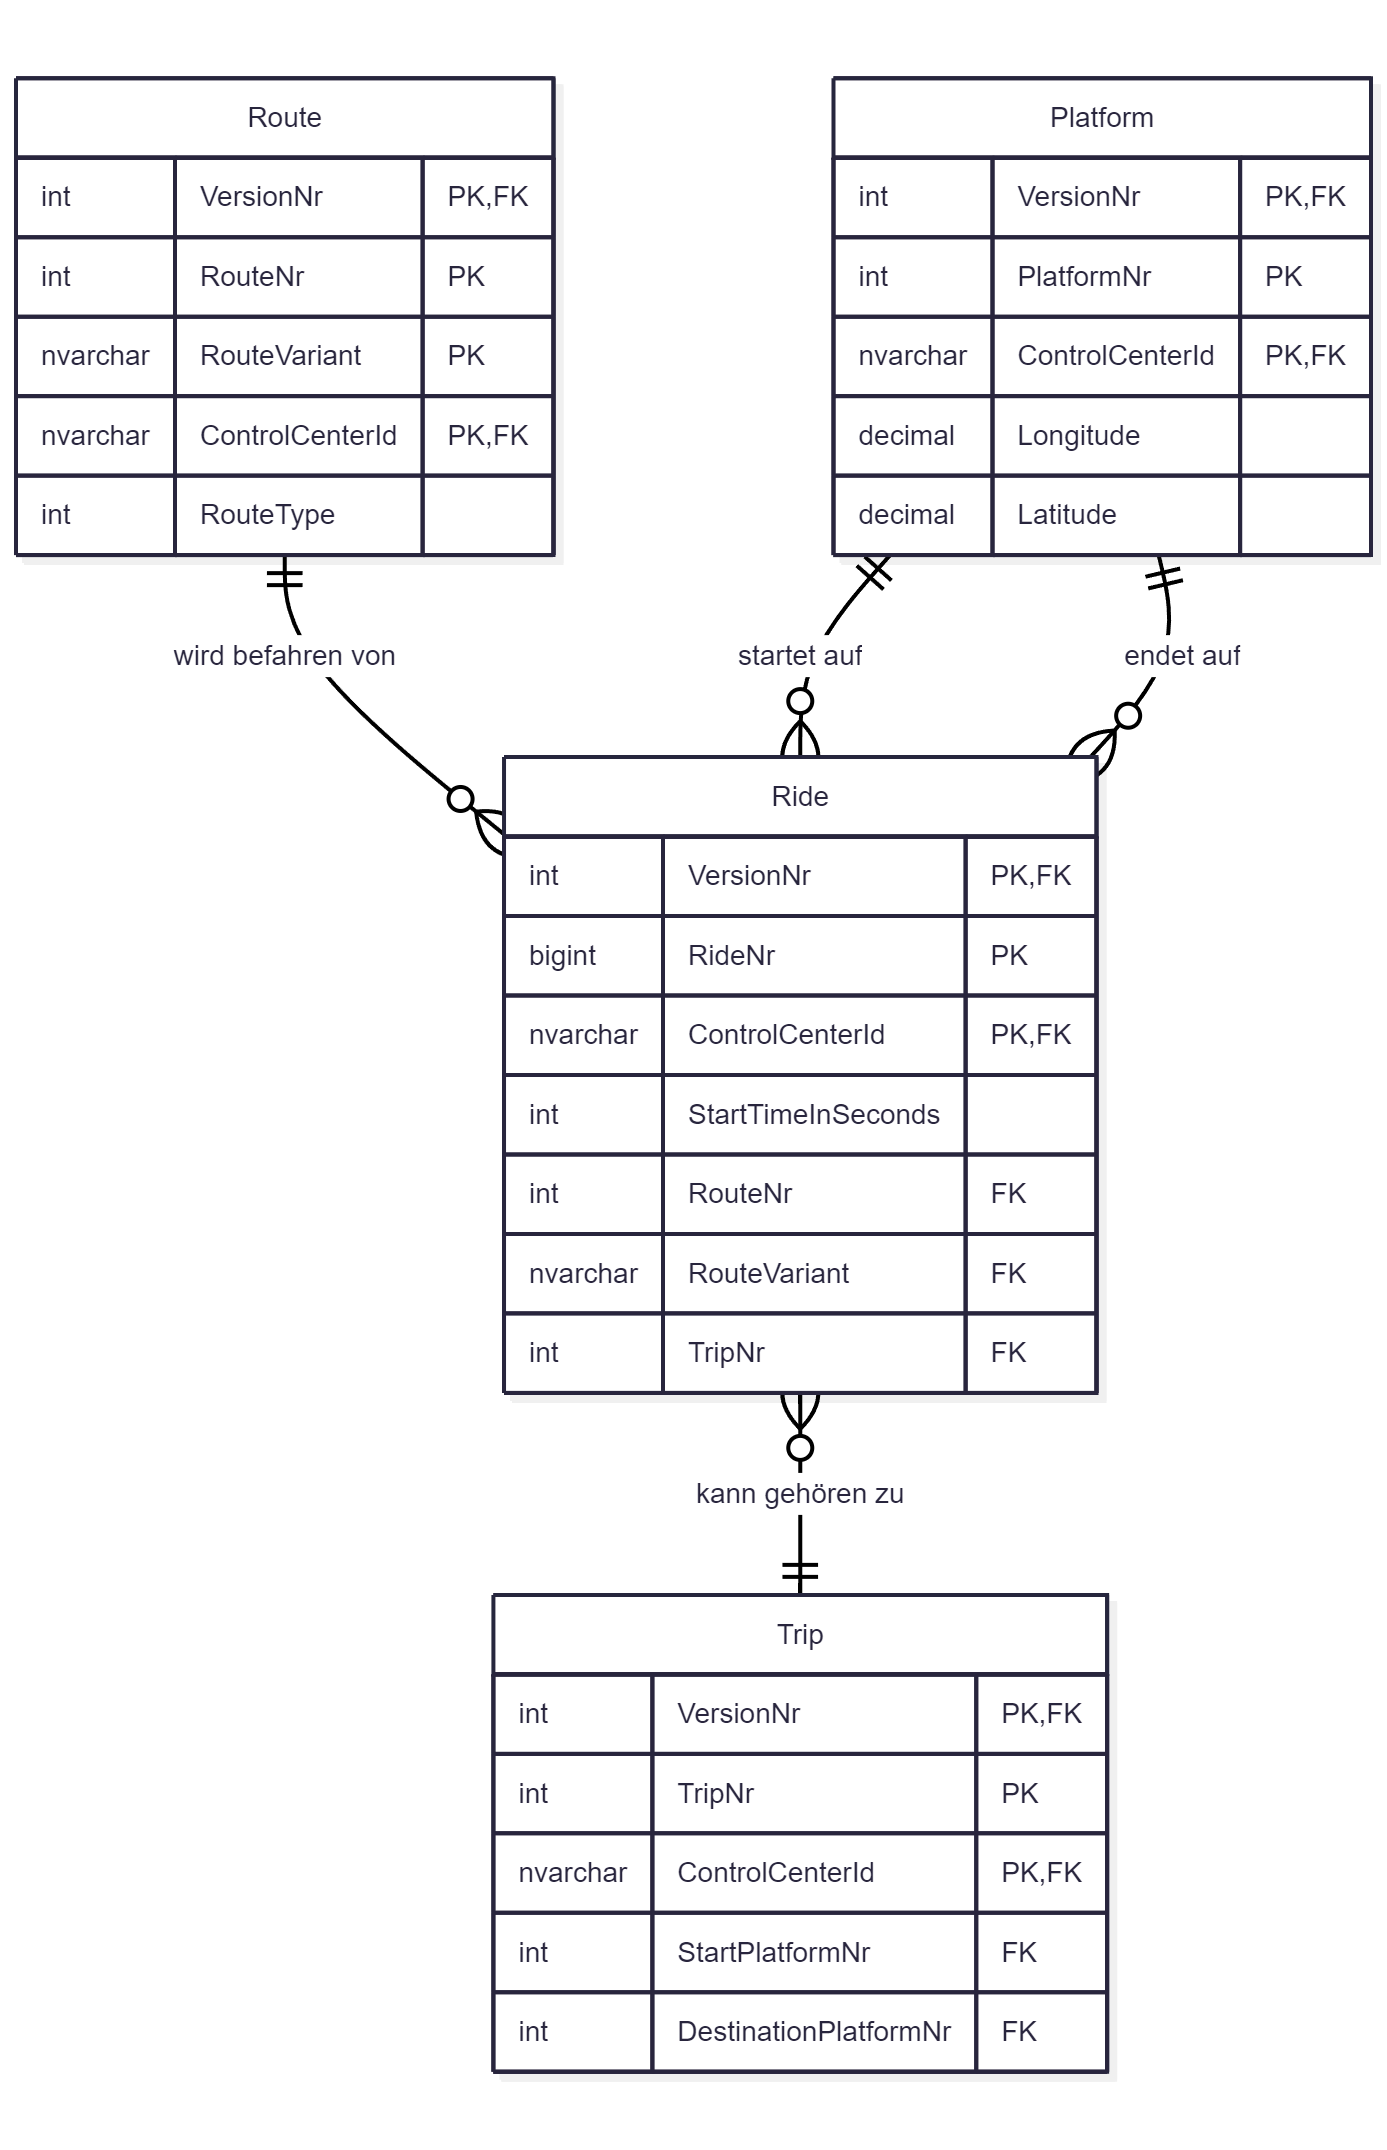
\includegraphics[width=0.8\textwidth]{transportation_system.png}
        \caption{Beziehungen von Umläufen und Fahrten}
        \label{fig:BeziehungenvonUmläufenundFahrten}
    \end{figure}

    Abbildung \ref{fig:BeziehungenvonUmläufenundFahrten} soll einen groben Überblick über das unmittelbar für diese Aufgabe benötigte Datenschema verschaffen. Für das Verständnis unwesentliche 
    Datenkomponenten und Beziehungen wurden weglassen. Die Entität "Route" ist in diesem Modell deswegen wichtig, da die Datenkomponente "RouteNr" die Art der Fahrt festlegt. Für Pausen oder nicht
    produktive
    Fahrten wird eine eigene Nummer vergeben. Zusätzlich ist bei jedem Umlauf ebenfalls jeweils eine Plattform-Entität (auch "Steig") als Start- und Endpunkt eingetragen. Dabei kann es sich bei den 
    Steigen um Sonderhaltepunkte wie beispielsweise Betriebshöfe handeln.

    Der Umlaufeditor besteht aus folgenden 3 Blazor-Seiten: 
    \begin{itemize}
        \item \emph{Sonderhaltepunkte}: Da Sonderhaltepunkte von den meisten Kunden nicht mit externen Tools erstellt werden und somit nicht beim Import neuer Versionen inbegriffen sind, 
                erlaubt diese Seite die Verwaltung und Erstellung neuer Sonderhaltepunkte.
        \item \emph{Umläufe}: Diese Seite stellt das Herzstück des Umlaufeditors dar. Hier können neue Umläufe erstellt und mit Fahrten versehen werden. Außerdem können bestehende Umläufe 
                als Vorlagen abgespeichert werden. 
        \item \emph{Vorlagen}: Hier können alle bestehenden Vorlagen eingesehen werden. Sollten für einen Umlauf mehrere Vorlagen bestehen oder Vorlagen in Zukunft nicht mehr durchführbar sein, können diese
                deaktiviert oder gelöscht werden.
    \end{itemize}

    Es sind zwar alle drei Seiten für den Einsatz des Umlaufeditors notwendig, jedoch verbirgt sich hinter der Seite \emph{Umläufe} die meiste Logik und sie stellt beim laufenden Betrieb das Herzstück dar.
    Der Prototyp der visuellen Grundstruktur der Seite ist in Abbildung \ref{fig:Umlaufeditor_konzept} zu sehen. Um die Seite implementieren zu können musste jedoch zunächst ein Konzept für den Ablauf 
    des Hinzufügens von Fahrten zu Umläufen erstellt werden. Das Ergebnis ist in vereinfachter Form als Ablaufdiagramms in Abbildung \ref{fig:Ablauf} zu sehen.

    \begin{figure}[H]
        \centering
        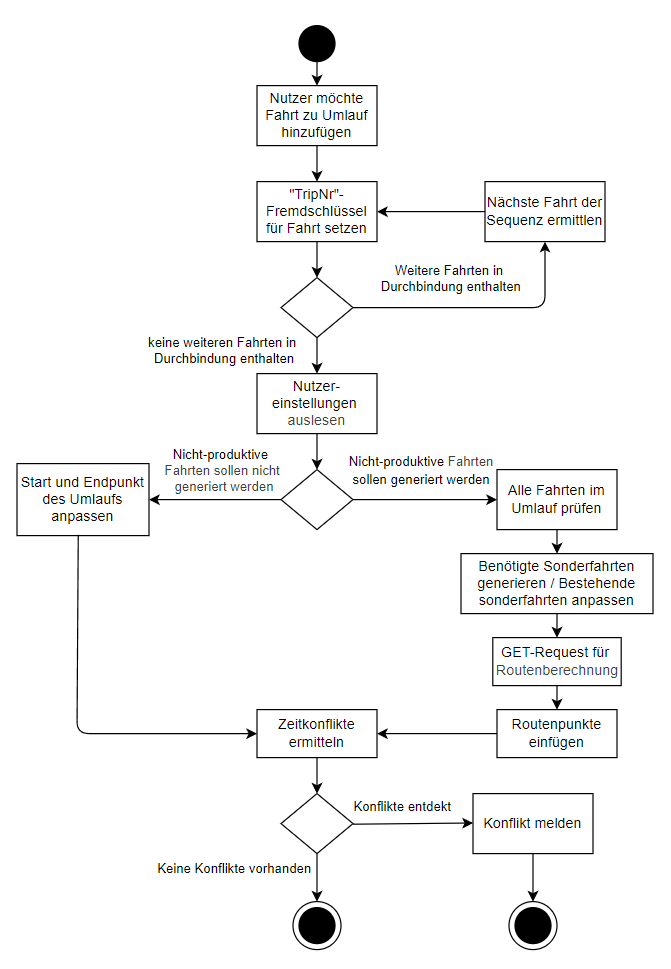
\includegraphics[width=0.8\textwidth]{Ablauf.png}
        \caption{Beziehungen von Umläufen und Fahrten}
        \label{fig:Ablauf}
    \end{figure}

     
\section{"ITCS"}\label{sec:itcs-design}
    Das Projekt \emph{"ITCS"} beinhaltet die SQL-Scripts die alle Änderungen an der Datenbank dokumentierten, um das Schema auf einer neuen Datenbank reproduzieren zu können. 
    Jedem dieser Scripte wird eine aufsteigende Versionsnummer zugeordnet. Diese Versionsnummer wird beim Aufruf des Scripts in eine eigene Datenbanktabelle eingetragen, um den Stand des Schemas
    eindeutig zu dokumentieren. Im Zuge des Praktikums wurde das Datenbank-Schema um einige neuen Tabellen erweitert und bestehende Tabellen um neue Spalten ergänzt. Das resultierte in
    einigen kleineren Create- und Alter-DDL-Scripten. Beispiele dafür sind die Erstellung einer neuen Tabelle für Sonderhaltepunkte oder das Einführen einer neuen Spalte bei Mandanten 
    die abspeichert welche Arten von Sonderfahrten für diese generiert werden sollen.

    Wie bereits erwähnt, liegt der Fokus des Projekts eigentlich auf den Import- und Export-Routinen. Diese werden verwendet, um Daten aus anderen Datenbanken oder Dateien mit dem 
    \emph{VDV-452}~\cite{VDV452} konformen \emph{"x10"}-Format in die ITCS-Datenbank zu importieren. Meist umfasst der Datentransfer eine neue Version des Fahrplans.
    Dieses Projekt nutzt jedoch nicht das \gls{efc} für den Zugriff auf Datenbanken, sondern verwendet die \emph{System.Data.SqlClient}-Bibliothek.
    Diese ist eine .NET-Bibliothek, die es ermöglicht, SQL-Server-Datenbanken zu verwalten 
    und zu manipulieren. Mithilfe dieser wurden ein eigener Datenbaken-Manager und ein attributbasiertes "Object-Relational Mapping" implementiert. Da alle Klassen dadurch von den 
    Basis-Klassen \texttt{Entity} und \texttt{VersionedEntity} erben, ist dieses Vorgehen eher restriktiv, jedoch auf den spezifischen Anwendungsfall optimiert.
    
    Die Routinen für den Import und Export lesen dann Daten aus einer Quelle, speichern diese im Arbeitsspeicher zwischen und schreiben sie dann entweder in eine Datenbank oder in eine Datei.
    Oftmals müssen die Daten dabei angepasst werden, da Quelle und Ziel unterschiedliche Datenschemen verwenden. 

    Der Datenbank-Zugriff und die Routinen wurden jedoch schon vor dem Praktikum implementiert und musste daher nur noch geringfügig angepasst werden, wenn neue Tabellen oder Spalten hinzugefügt wurden.
    Die Anpassungen beschränkten sich dabei auf das Hinzufügen von neuen Methoden im Datenbank-Manager und neuer Domain-Model-Klassen, die die neuen Tabellen repräsentieren.
    
    Im Praktikum wurde dieses Projekt hauptsächlich verwendet, um Methoden, deren Logik in anderen Projekten wiederverwendet werden können sollte, zu implementieren. 
    Dies umfasst beispielsweise die Generierung von Daten wie Metadaten für Sonderfahrten. Wenn die Koordinaten der Sonderhaltepunkte für die neu generierte Sonderfahrt definiert wurden,
    sollte ein \emph{HTTP}-Request an eine externe API gesendet werden, um berechnete Strecke inklusive Fahrtbeschreibung in Form von Wendepunkten zu erhalten. Diese 
    Informationen wird dann aus der \emph{JSON}-Response extrahiert und in der Datenbank gespeichert. Fahrtzeit und -länge werden 
    später für die Ermittlung von Konflikten zwischen Fahrten in Umläufen benötigt. Die Streckenbeschreibung wird für eine 
    visuelle Darstellung der Fahrt benötigt. Diese ist aber nicht mehr Teil des Praktikums.

\chapter{Implementierung}\label{ch:Implementierung}
\section{Implementierung "ITCS-Management"}\label{sec:ImplementierungITCS-Management}
    Die Benutzeroberflächen der \emph{ITCS-Management}-Anwendung wurden wie bereits erwähnnt mit Blazor implementiert. Dabei werden pro Seite 
    zwei Dateien angelegt. Eine \texttt{.razor}-Datei, die das Layout der Seite über eine XML-ähnliche Syntax definiert
    und eine \texttt{razor.cs}-Datei, die als \texttt{partial} markiert werden muss und alle benötigten Methoden und Logik hinter der Seite enthält. Manchmal ist die Verwendung einer \texttt{razor.css}-Datei 
    auch sinnvoll, um die Seite zu stylen. Die Logic und die Css-klassen könnten zwar auch inder der \texttt{.razor}-Datei definiert werden,
    aber das würde die Übersichtlichkeit stark verringern. 
    
    Der Datenbankzugriff erfolgt über mehrere Schichten. \emph{Repositories} sind dafür zuständig, 
    die Daten aus der Datenbank zu laden und zu speichern. Sie führen normalerweise nur grundlegende Interaktionen mit der Datenbank über den Datenbank-Kontext des \gls{efc} aus.
    Diese \emph{Repositories} werden dann von den \emph{Services} verwendet, die die Logik der Anwendung enthalten. Ein großer 
    Vorteil der Verwendung von Blazor im Vergleich zu anderen Frontend-Technologien wie Angular oder React ist, dass die gesamte Logik der Anwendung in
    C\# geschrieben werden kann. Dadurch werden sind keine HTTP-Endpoints benötigt da auf die Daten des Teilprojekts für den Datenbankzugriff direkt zugegriffen werden kann.
    Die Services und Repositories wurden dann in der \texttt{Program.cs}-Datei der Anwendung für die Dependency-Injection registriert,
    damit sie in den Blazor-Komponenten verwendet werden können.

    Für die Darstellung der Daten im Frontend wurde auf UI-Komponentenbibliothek \emph{Radzen Blazor}~\cite{radzen} zurückgegriffen. 
    Diese Bibliothek bietet eine Vielzahl an vorgefertigten Komponenten, die das Erstellen von Benutzeroberflächen erleichtern.
    
    \begin{program} [H]
        \caption{Ermittlung der zu generierenden Fahrten}
        \label{prog:RideGeneration}
    \begin{CsCode}[numbers=left]
RideViewItem pRide = null;
foreach (RideViewItem cRide in sortedRides)
{
    if (pRide is null){ pRide = cRide; continue; }

    int previousEndTime = pRide.StartTimeInSeconds + pRide.DriveTimeInSeconds;
    int timeBetweenRides = cRide.StartTimeInSeconds - previousEndTime;

    if (!IsSpecialStopPoint(pRide.DestinationLocationTypeNr) &&
        !IsSpecialStopPoint(cRide.StartLocationTypeNr))
    {
        bool isSameLocation = AreLocationsEqual(
            pRide.DestinationLocationNr, pRide.DestinationLocationTypeNr,
            cRide.StartLocationNr, cRide.StartLocationTypeNr);

        if (!isSameLocation && this.generateNonProductiveRides)
        {
            RideViewItem existingEmptyRide = existingGeneratedRides
                .FirstOrDefault(r => r.RouteNr == 9999 &&
                    r.StartLocationNr == pRide.DestinationLocationNr &&
                    r.StartLocationTypeNr == pRide.DestinationLocationTypeNr &&
                    r.DestinationLocationNr == cRide.StartLocationNr &&
                    r.DestinationLocationTypeNr == cRide.StartLocationTypeNr);

            if (existingEmptyRide is not null)
            {
                neededRides.Add(existingEmptyRide.RideNr);
                int newStartTime = pRide.StartTimeInSeconds + 
                    pRide.DriveTimeInSeconds + pRide.RideStopTimeInSeconds;
                if (existingEmptyRide.StartTimeInSeconds != newStartTime)
                    await this.UpdateRideStartTime(existingEmptyRide, newStartTime);
            }
            else
                await this.GenerateForEmptyRide(pRide, cRide, generator, trip);
        }
        else if (isSameLocation && timeBetweenRides > minimumBreakTime && 
                    this.generateBreaks &&
                    IsNoSpecialRide(pRide) && !IsConnectThrough(pRide, cRide))
        {
            RideViewItem existingBreak = existingGeneratedRides
                .FirstOrDefault(r => r.RouteNr == 9989 &&
                    r.StartLocationNr == pRide.DestinationLocationNr &&
                    r.StartLocationTypeNr == pRide.DestinationLocationTypeNr);

            if (existingBreak is not null)
            {
                neededRides.Add(existingBreak.RideNr);
                int newStartTime = pRide.StartTimeInSeconds + 
                    pRide.DriveTimeInSeconds + pRide.RideStopTimeInSeconds;
                if (existingBreak.StartTimeInSeconds != newStartTime)
                    await this.UpdateRideStartTime(existingBreak, newStartTime);
            }
            else
                await this.GenerateBreak(pRide, trip, generator);
        }
    }
}\end{CsCode} \end{program}

    In Programm~\ref{prog:RideGeneration} ist ein Ausschnitt der Methode zu sehen, die für die Ermittlung der zu generierenden Fahrten zuständig ist. Um genauer zu sein,
    handelt es sich um den Teil der die zu generierenden Leerfahrten und Pausen ermittelt. Zunächst werden dafür allen Fahrten in dem Umlauf nach ihrer Startzeit sortiert.
    Anschließend wird in einer Schleife über alle sortierten Fahrten iteriert wobei jede Fahrt gemeinsam mit der vorherigen betrachtet wird. Sind der Zielpunkt der vorherigen Fahrt
    und der Startpunkt der aktuellen Fahrt nicht gleich, wird eine Leerfahrt benötigt. Um unnötige Generierungen zu vermeiden, wird zunächst geprüft, ob eine Leerfahrt bereits existiert.
    Sollte dies der Fall sein, wird diese Fahrt in die Liste der benötigten Fahrten aufgenommen und die Startzeit der Leerfahrt aktualisiert, falls sie sich geändert hat.
    Sind der Zielpunkt der vorherigen Fahrt und der Startpunkt der aktuellen Fahrt gleich, wird geprüft, ob eine Pause generiert werden soll. Solche Sonderfahrten werden nur generiert, wenn
    der Kunde dies explizit in den Einstellungen aktiviert hat und wenn es sich bei beiden Fahrten nicht um Sonderfahrten handelt. Sollte es um Anschlussfahrten gehen,
    werden ebenfalls keine Pausen generiert.

\section{Implementierung "ITCS"}\label{sec:ImplementierungITCS}
    
    Das Projekt \emph{ITCS} wurde um die Klasse \texttt{EntityGenerator} erweitert. Diese Klasse wird mit einem Datenbank-Connetion-String initialisiert 
    und kann dann verwendet werden, um Daten in die Datenbank zu generieren. Für manche Operationen wurde auf den bereits erwähnten Datenbank-Manager zurückgegriffen. 
    Die Transaktionsverwaltung wurde aber für jede Methode selbst implementiert, da der Datenbank-Manager nicht für alle Operationen geeignet ist. Oftmals 
    wurden Operationen direkt als SQL-Statements ausgeführt. 
    Die Methoden von \texttt{EntityGenerator} sollten als Bibliothek in anderen Projekten verwendet werden können.
    \begin{program} [H]
        \caption{Ermittlung der zu generierenden Fahrten}
        \label{prog:RideGeneration}
    \begin{CsCode}[numbers=left]
public virtual int GenerateCourseNr(string ccid, int routeNr)
{
    if (string.IsNullOrEmpty(ccid))
        throw new ArgumentException("ControlCenterId darf nicht leer sein.",
             nameof(ccid));

    using ITCSDatabaseManager itcsDbManager = new(this.connectionString, 
        this.commandTimeout);
    var config = itcsDbManager.GetControlCenterConfiguration(ccid) ??
        throw new ArgumentException(
            $"Keine Konfiguration für '{ccid}' gefunden.", nameof(ccid));

    int courseNoLength = config.CourseNoLength > 0 ? config.CourseNoLength : 3;

    int maxCourseValue = 899;
    if (courseNoLength > 0)
        maxCourseValue = (int)Math.Pow(10, courseNoLength) - 101;

    List<VersionValidity> versions = 
        itcsDbManager.GetCurrentAndFutureVersions(ccid);
    if (versions.Count == 0)
        throw new InvalidOperationException(
            "Es wurden keine aktuellen oder zukünftigen Versionen gefunden.");

    int highestCourseNr = 0;
    int currentPrefix = routeNr;
    bool found = false;
    while (!found && currentPrefix >= routeNr - 10)
    {
        int internalHighestCourseNr = 0;
        foreach (VersionValidity version in versions)
        {
            IList<Ride> rides = itcsDbManager.GetRidesByRoute(ccid,
                version.VersionNr, currentPrefix, null);

            foreach (Ride ride in rides)
                if (ride.CourseNr > highestCourseNr && 
                    ride.CourseNr % currentPrefix <= maxCourseValue)
                    internalHighestCourseNr = ride.CourseNr;
        }
        if (internalHighestCourseNr % currentPrefix < maxCourseValue)
        {
            highestCourseNr = internalHighestCourseNr;
            found = true;
            break;
        }
        currentPrefix--;
    }
    if (!found)
        throw new InvalidOperationException("keine gültige Kursnummer gefunden.");

    return (currentPrefix * (int)Math.Pow(10, courseNoLength)) + 
        ((highestCourseNr + 1) % currentPrefix);
}\end{CsCode} \end{program}
\chapter{Testen}\label{chap:testen}
    Das Testen des im Rahmen des Praktikums erstellten Codes war nicht Schwerpunkt der Arbeit des Praktikanten. Meistens wurden deswegen vor allem im Projekt \emph{"ITCS-Management"} nur 
    manuelle Integrationstests über das UI durchgeführt. Bei Bedarf wurden auch Sql-Statements direkt in der Datenbank ausgeführt, um die Korrektheit der Daten zu überprüfen. 
    Weitere Tests wurden von anderen  Mitarbeiter der Firma durchgeführt ohne direkte Beteiligung des Praktikanten. Sollten 
    Fehler aufgetreten sein, wurden diese in einem Bug-Tracker dokumentiert und vom Praktikanten später behoben.

    Bei zwei verschiedenen Aufgaben im Projek \emph{"ITCS"} wurden jedoch explizit automatisierte Tests durch den Praktikanten gefordert.
    Diese wurden mit der \emph{xUnit}-Bibliothek~\cite{xunit}, einer weit verbreiteten Testbibliothek für .NET-Anwendungen, erstellt.
    Für das Mocken von Datenbankzugriffen wurde die \emph{Moq}-Bibliothek~\cite{moq} verwendet. Diese ermöglicht es, Objekte zu erstellen, die das Verhalten von Abhängigkeiten simulieren.
    Einerseits wurden dabei Unit-Tests für eine Methode erstellt, die für Fahrten neue \texttt{CourseNr}-Werte generiert. Diese Werte sind zwar nicht Teil des Primärschlüssels, sind jedoch 
    für weitere Verwendung der Daten auf anderen Systemen wichtig und müssen aus diesem Grund eindeutig sein und eine bestimmte Struktur aufweisen. 

    \begin{program} [H]
        \caption{Beispiel eines Unit-Tests für die Generierung von CourseNr-Werten}
        \label{prog:UnitTest}
    \begin{CsCode}[numbers=left]
[Fact]
public void GenerateCourseNrIgnoresOutOfRangeValuesWhenGeneratingNextNumber()
{
    Mock<ITCSDatabaseManager> dbMock = new("conn", 30) { CallBase = true };
    dbMock.Setup(m => m.GetControlCenterConfiguration("cc1"))
        .Returns(new ControlCenterConfiguration { CourseNoLength = 3 });
    dbMock.Setup(m => m.GetCurrentAndFutureVersions("cc1"))
        .Returns(new List<VersionValidity> { new() { VersionNr = 1 } });

    dbMock.Setup(m => m.GetRidesByRoute("cc1", 1, 9999, null))
        .Returns(new List<Ride> {
            new() { CourseNr = 9999005 },
            new() { CourseNr = 9999950 },
            new() { CourseNr = 9999003 }
        });

    TestEntityGenerator generator = new(dbMock.Object);
    int result = generator.PublicGenerateCourseNr("cc1", 9999);
    Assert.Equal(result, Is.EqualTo(9999006));
}\end{CsCode}
    \end{program}

    In Programm~\ref{prog:UnitTest} ist ein Beispiel eines Unit-Tests für die Generierung von CourseNr-Werten zu sehen. 
    Anfangs wird ein Mock-Objekt für die Datenbank erstellt, das die Abhängigkeit von der echten Datenbank simuliert. Dabei wird für 
    einzelne Methodenaufrufe das erwartete Verhalten festgelegt. Anschließend wird die zu testende Methode aufgerufen und das Ergebnis überprüft.

    Die weiteren mit Tests versehenen Methoden generieren oder verändern Daten in der Datenbank, sollten bestimmte Objekte wie Betriebshöfe Sonderhaltepunkte in die
    Datenbank eingefügt oder modifiziert werden. Da sie für den Datenbankzugriff auf sehr viele eigens dafür erstellte Sql-Statements zurückgreifen, wurden sie in Integrationstests 
    mit direkten Abhängigkeiten von einer Test-Datenbank getestet. Benutzt wurde dafür eine Firmeneigene Test-Datenbank, die regelmäßig mit den aktuellen Daten der Produktionsdatenbank gefüllt wird.
    Die Tests wurden aber dennoch so gestaltet, dass sie nur an das Datenschema gebunden sind und nicht an die konkreten Daten.
    Es wurde ebenfalls \emph{xUnit} verwendet und die Tests ähneln dem Beispiel in Programm \ref{prog:UnitTest}, nur dass hier die Datenbankabfragen nicht gemockt, sondern 
    direkt ausgeführt werden und alle erstellten Objekte abgespeichert und anschließend wieder gelöscht werden, um die Test-Datenbank nicht zu verändern.
\chapter{Zusammenfassung und Erfahrungen}\label{ch:ZusammenfassungundErfahrungen}
    Da der genaue Umfang der geplanten Arbeit des Praktikums von der Firma nie genau festgelegt oder kommuniziert wurde,
    ist es schwierig zu festzustellen, ob die Arbeit nach den Erwartungen der Firma verlaufen ist. Es wurden nicht alle Aufgaben am Taskboard abgeschlossen. 
    Viele Aufgaben wurden jedoch während der aktiven Arbeit an den Anwendungen neu angelegt, wobei auch klar erkennbar war, dass
    diese Aufgaben nicht im ursprünglichen Plan enthalten waren. Das Feedback der Betreuer war auch durchwegs positiv. Alle wichtigsten Features des Herzstückes 
    der Arbeit, der \emph{Umlaufeditor}, wurden implementiert und funktionieren wie geplant.

    Es müssen jedoch noch einige Integrationstests durchgeführt werden, um die Qualität der Software zu gewährleisten. Auch sollten manche Dinge von der 
    Firma noch genauer überdacht bzw. überarbeitet werden. Beispielsweise returniert der Dienst zur Ermittlung der Strecken für
    Sonderfahrten keinen spezifischen Fehlercode, sondern nur \texttt{500 Internal Server Error}. Da während des Praktikums kein Zugriff keine Einsicht in den Quellcode
    des Dienstes möglich war, war es nicht möglich genau zu ermitteln, warum manche Fehler bei der Generierung der Strecken auftreten.

    Durch die Arbeit in der Firma konnte ich viele neue Erfahrungen sammeln. Ich erlangte wichtige Einblicke in die Arbeit eines agilen Softwareentwicklungsteams.
    Dazu kann auch gehören, dass neue Anforderungen während der Entwicklung definiert werden oder bestehende Anforderungen stark verändert werden.
    Auch im Umgang mit verschiedenen Technologien konnte ich mein Wissen erweitern. So habe ich zum Beispiel sehr viel über die Arbeit mit Blazor gelernt. An der FH 
    wurde Blazor nämlich nur kurz in einer Vorlesung besprochen, ohne viel praktische Erfahrung damit zu sammeln. Auch die starke Verwendung von \gls{efc} konnte mir 
    helfen, meine Kenntnisse in diesem Bereich zu erweitern. 
    Man kann zusammenfassend sagen, dass ich durch dieses Praktikum sowohl meine technischen Fähigkeiten als 
    Softwareentwickler erweitern konnte als auch Erfahrungen über die Arbeit in einem Entwicklerteam sammeln konnte. Diese wichtigen Einblicke in die Arbeitswelt
    der Softwareentwicklung werden mir in meiner zukünftigen beruflichen Karriere sicherlich von großem Nutzen sein.


% \chapter{Das Unternehmen}

% Umfang: 1--2 Seiten
% %%%-----------------------------------------------------------------------------

% \chapter{Projekte und Tätigkeiten während des Praktikums}

% Umfang: 2--3 Seiten (Projektziel(e), Projektumfeld)

% %%%-----------------------------------------------------------------------------
     
% \chapter{Projektbeispiele}

% Umfang: 5--6 Seiten (Umsetzung, grober Terminplan, Ergebnisse,
% Qualitätssicherungsmaßnahmen)

% %%%-----------------------------------------------------------------------------

% \chapter{Erfahrungen und Zusammenfassung}

% Umfang: 1--2 Seiten

%%%-----------------------------------------------------------------------------
\backmatter        % Schlussteil (nur bei Verwendung des Quellenverzeichnisses)
%%%-----------------------------------------------------------------------------

\MakeBibliography % Quellenverzeichnis (sofern notwendig, sonst weglassen)

\end{document}
